\chapter{How \textsc{Becca}'s reinforcement learner works}
\label{actor_chapter}

\textsc{Becca}'s reinforcement learner starts with the set of feature activities passed from the feature extractor at each time step. (See Figure~\ref{becca_reinforcement_learner}.) It attends to one of the features, passes the attended feature together with the full feature activities and reward to the model, and chooses an action to pass to the world. Each of these steps is described in detail below  

\begin{figure}
\centering
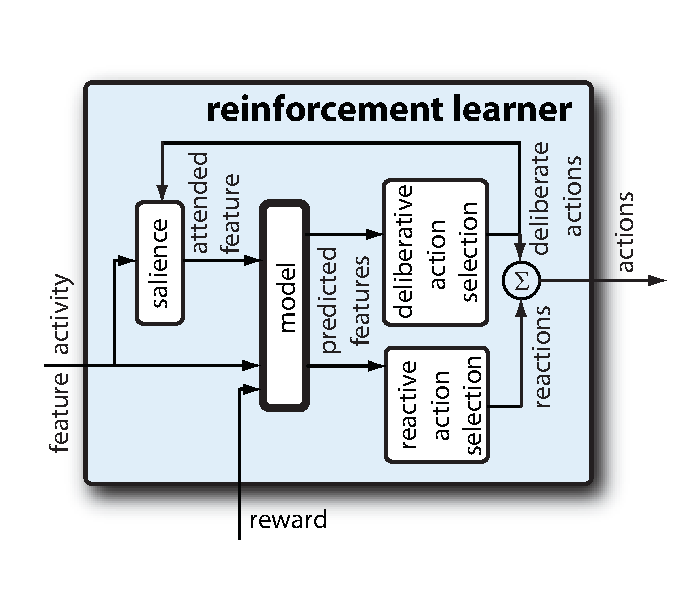
\includegraphics[height=11cm]{figs/becca_reinforcement_learner.eps}
\caption{Block diagram of \textsc{Becca}'s reinforcement learner.}
\label{becca_reinforcement_learner}
\end{figure}

\section{Attention}
Each of the feature primitives, the actions, and the created features is eligible for attention. The most salient feature in this set is attended at each time step. In practice, this means that in the array representing attention, the attended feature value is set to one and all others are set to zero. The criteria for salience are still under heavy development, and are likely to change in future versions of \textsc{Becca}, but currently they are as follows. There are four contributing factors to the salience, $\omega$, of a feature. They are the feature's activity, the feature's reliability in predicting reward, how often and recently that feature has been attended, and some random noise:

\begin{equation}
\omega = f _\omega (1 - \beta_\omega) \nu_\omega
\end{equation}

The calculation of $f_\omega$ is explained later, in section~\ref{reliability}, since it references the model which has not yet been described. Salience fatigue is a mechanism to promote attention sharing among features. When a feature is attended its fatigue is incremented by one. Then at each time step, the fatigue is decayed:

\begin{equation}
f_{\omega_{t+1}} = f_{\omega_t}  D_{fdr}
\end{equation}

A small amount of random noise is added to the feature activities to act as a tie breaker between features that may be active at exactly the same level. This condition occurs commonly when working with simulated worlds. 

$\nu_\omega$ is a multiplicative noise term of the form

\begin{equation}
\nu_\omega= 1 + \frac{D_{san} }{ \mathcal{U}(0,1)}
\end{equation}

where $ \mathcal{U}(0,1)$ is the uniform distribution on the interval $[0,1)$ and $D_{san}$ is the characteristic salience noise level. Note that the $\frac{1}{x}$ structure of the noise gives is an extremely long tail. The noise will occasionally dominate all other aspects of the salience process

The most salient feature is attended, unless a deliberate action was taken on the previous time step, in which case that action is attended. 

Future candidates for salience calculation include:

\begin{itemize}
\item {\bf Recency}  Recently attended features would be penalized. Rarely observed features would be more salient.
\item {\bf Surprise} Expected features would be less likely to be attended. Unexpected ones would be more salient.
\item {\bf Goal relevance} Features that have been selected as intermediate goals would be more salient.
\end{itemize}


\section{Model}
The model is the core of the reinforcement learner. It contains snippets of the agent's experience in the form of {\em transitions}. The collection of transitions constitutes the whole of the agent's experience. Each is a small piece of memory. Taken together, the set of transitions is a distillation of the agent's interactions with its world. On the agent's first time step, the model is empty, but as it gathers experience it gradually populates its model, increasing the fidelity of its representation of the world. 

\subsection{Transition structure}

Each transition is of the form (\texttt{context}, \texttt{cause}, \texttt{reward}, \texttt{effect}) and captures a short sequence of events. (See Figure~\ref{transition_structure}.) Contexts, causes, and effects may contain state or action information or both.

\begin{figure}
\centering
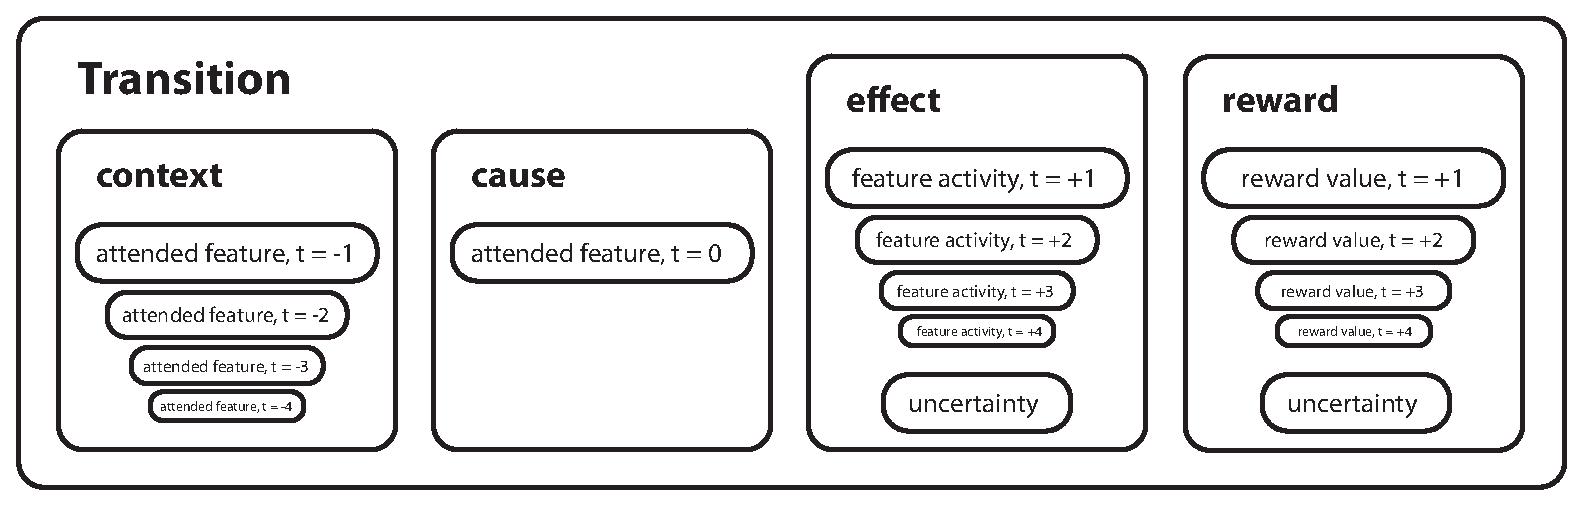
\includegraphics[height=4cm]{figs/transition.eps}
\caption{The structure of a transition in the model.}
\label{transition_structure}
\end{figure}

Transitions also contain a quantification of the uncertainty in both effects and rewards. \texttt{context}--\texttt{cause} pairs uniquely define a transition. The effect and reward that results from a given context and cause may vary a great deal each time the transition is observed. Rewards and effects are the expected value of starting in a given context and executing a given cause. The reward uncertainty and effect uncertainty are the expected error on those predictions.

 
\subsubsection{Context}
Context is a combination of the several most recent attended features. It captures the agent's recent history of attention, summarizing the most salient parts of its world.
Specifically, if the current time step is labeled $t_{0}$, the context includes the attended features from $t_{-D_{trl}}$ to $t_{-1}$, where $D_{trl}$ is a user-defined integer, typically small. The attended features are decayed according to their age, as follows:

\begin{equation}
\mathbf{h}^\prime_{t_0-i} =  \mathbf{h}_{t_0-i} D_{tdr}^{i-1} 
\end{equation}

where $ \mathbf{h}_{t_0-i} $ is the magnitude of the attended feature at time step $t_0-i$ (always 1 in the current implementation), $\mathbf{h}^\prime_{t_0-i}$ is the decayed magnitude of the attended feature, and $D_{tdr}$ is between zero and one.

The context, $\mathbf{c}$, is the the combination of all the decayed attended features. In the case where the same feature has been attended more than once within the last $D_{trl}$ time steps, the decayed magnitudes are added in a nonlinear way, such that the resulting magnitude is guaranteed to be less than or equal to one: 

\begin{equation}
\mathbf{c} = g \left( \sum\limits_{i = 1} ^ {D_{trl}} g^{-1}(\mathbf{h}^\prime_{t_0-i}) \right )
\end{equation}

The result is a bounded sum operation that ensures the magnitude of the result will always lie between zero and one, given that its operands did.


\subsubsection{Cause}
The cause is simply the attended feature at the current time step, $t_0$. It may be an action, in which case the \texttt{context}--\texttt{cause}--\texttt{effect} sequence resembles a state--action--state tuple. But it can also be a primitive feature or created feature, in which case the transition represents an observed sequence of features, rather than a record of the agent's interaction with the world

\begin{equation}
\mathbf{d} = \mathbf{h}_{t_0}
\end{equation}
 
\subsubsection{Effect}
The effect is the combination of the feature activities from $t_1$ through $t_{D_{trl}}$. These are decayed and summed the same way attended features are decayed and summed to produce contexts, only in the opposite time direction, with immediate feature activity being undecayed and future feature activities increasingly decayed:

\begin{equation}
\mathbf{e} = g \left( \sum\limits_{i = 1} ^ {D_{trl}} g^{-1}(\mathbf{f}_{t_0+i} D_{tdr}^{i-1} ) \right )
\end{equation}
 

Effects are composed of feature activities, rather than attended features because they contain a more complete picture of the effects of a given context and cause. Since the transition is identified by the uniqueness of the context and cause alone, the effect can contain a lot of information without making the transition overly specific. 

\subsubsection{Effect uncertainty}
Each time a transition is observed, the effect is updated to reflect the result. It can be the case that a wide variety of effects may result from the same context and cause. The effect captures something resembling the average of these effects. The effect uncertainty provides an estimate of the expected difference between the effect and effects that will result from future encounters with the same context and cause. 

The effect uncertainty is useful in making predictions. Particularly when the uncertainty is low, deviations from expected effects can be flagged as highly salient.

\subsubsection{Reward}
The reward that results from each observation of the transition is used to update an estimate of the transition's expected reward. This quantity explicitly describes the desirability of the transition, a value made use of in planning.

The reward associated with a transition combines reward signal received over the next several time steps, decayed and summed in the same way as the effect, except that it is not re-mapped to guarantee that its result falls on $[-1, 1]$. In fact, rewards can be any real value, as can their summed and decayed sequences. The summed reward produces a trace which allows the transition to represent outcomes of the context and cause that are desirable but may be slightly delayed. 

\subsubsection{Reward uncertainty}
As with the effect, the reward uncertainty is the expected value of the difference between the expected reward and future observations of reward. It is a quantification of confidence in the reward estimate.

\subsubsection{Count}
The count is a reflection of the number of times a transition has been observed or has been used in planning. It determines the update rate for transitions and whether and when they are forgotten.

\subsection{Adding transitions}
At each time step, the model compares the current context and cause to that of all of its existing transitions.
A matching transition is one that has both 
\begin{enumerate}
\item the same cause and 
\item a sufficiently similar context.
\end{enumerate}

Context similarity is determined by treating all the features (including basic features and actions) as dimensions of the same space. Both the current context and the transition context are vectors in that space. 
The similarity measure, $\sigma$, is based on the element-wise difference between two arrays. If $\sigma(\mathbf{a},\mathbf{b})$ is the similarity between two arrays $\mathbf{a}$ and $\mathbf{b}$, then:

\begin{equation}
\sigma(\mathbf{a},\mathbf{b}) = 2^{-\sum\limits_i |a_i - b_i|} 
\label{similarity_simple}
\end{equation}

over all the elements $i$ in the arrays.

% here is the verbiage that goes with the more complex angle-based similarity measure
\iffalse
The similarity measure, $\sigma$, is based on the angle, $\theta$, between two vectors. If $\sigma(\mathbf{a},\mathbf{b})$ is the similarity between two vectors $\mathbf{a}$ and $\mathbf{b}$, then:

\begin{equation}    
\sigma(\mathbf{a},\mathbf{b}) = 1 - \frac{\theta}{\pi/2}
\label{similarity}
\end{equation}

This similarity measure has several desirable properties:
\begin{enumerate}
\item $\sigma(\mathbf{a},\mathbf{b}) = \sigma(\mathbf{b},\mathbf{a})$ It is symmetric.
\item $\sigma(\mathbf{a},\mathbf{b})$ is on $[0,1]$
\item If $\mathbf{a}$ and $\mathbf{b}$ share no nonzero elements, $\sigma(\mathbf{a},\mathbf{b}) = 0$
\item $\sigma(\mathbf{a},\mathbf{b}) = 1$ if and only if $\mathbf{a} = c \mathbf{b}$, where $c$ is a constant greater than 0, that is, if $\mathbf{a}$ and $\mathbf{b}$ are pointing in exactly the same direction.
\end{enumerate}
\fi

Two contexts $\mathbf{c}_a$ and $\mathbf{c}_b$ are considered sufficiently similar if $\sigma(\mathbf{c}_a,\mathbf{c}_b) > D_{sit}$, where the similarity threshold $D_{sit}$ is between 0 and 1, typically closer to 1 than 0.

If more than one matching transition is in the library, the one with the highest similarity wins. If no matching transitions are in the library, the new transition is added. This requires waiting until the full effect and reward has been observed, so there is a delay of $D_{trl}$ time steps before new transitions are added to the model.

\subsection{Modifying transitions}
In instances where the current context and cause do match an existing transition, the effect, reward, and their uncertainties are updated based on the new observation.

When a transition is updated, the following events occur:
\begin{itemize}
\item The count is increased by one.
\item The effect is modified to incorporate the newly observed effect.
\item The effect uncertainty is modified to incorporate the difference between the effect and the newly observed effect.
\item The reward is modified to incorporate the newly observed reward.
\item The reward uncertainty is modified to incorporate the difference between the reward and the newly observed reward.
\end{itemize}

In order to perform the updates, an update rate, $\rho_e$ is first calculated:

\begin{equation}
\rho_e = \min(1.0, D_{tur}+ \frac{1 - D_{tur}}{n})
\end{equation}

where $n$ is the count of the transition being updated and $D_{tur}$ is a real value between zero and one. For large values of $n$, $\rho_e$ approaches $D_{tur}$. It can be considered a lower bound on the update rate. For values of $D_{tur}$ close to zero, transitions cease to change significantly after they have been observed many times. For higher values of $D_{tur}$, they remain malleable throughout their lifetimes.

Each feature in the effect is updated, shifted toward the newly observed value by a fraction, $\rho_e$, of the way. For an existing effect feature value, $e_i$, and a new effect observation $\tilde{e}_i$ the updated feature value, $e^\prime_i$ is given by:

\begin{eqnarray}
\Delta e_i &= &\tilde{e}_i  - e_i \\
e^\prime_i &=& e_i + \rho_e \Delta e_i
\end{eqnarray}

By the same mechanism, the effect uncertainty features, $e_{\epsilon_i}$, are updated using $\Delta e_i$:

\begin{eqnarray}
\Delta e_{\epsilon_i} &=& |\Delta e_i|  - e_{\epsilon_i}\\
e_{\epsilon_i}^\prime &=& e_{\epsilon_i} + \rho_e \Delta e_{\epsilon_i}
\end{eqnarray}

Reward, $r$, and reward uncertainty, $r_\epsilon$ are updated using the same mechanism as well, with the same update rate:

\begin{eqnarray}
\Delta r &= &\tilde{r} - r \\
r^\prime &=& r + \rho_e \Delta r \\
\Delta r_\epsilon &=&|\Delta r| -  r_\epsilon \\
r_\epsilon^\prime &=& r_\epsilon + \rho_e \Delta r_\epsilon
\end{eqnarray}

When a transition is first added and no previous values of $\mathbf{e}$ and $r$ exist from which to calculate  $\mathbf{e}_\epsilon$ and $r_\epsilon$, those values are all initialized to $D_{iun}$. 

\subsection{Forgetting}
Every new transition encountered is stored in the model, but many transitions are observed only rarely and result in neither reward nor punishment. These are periodically removed from the model in order to keep \textsc{Becca}'s processing speed up and its space requirements modest. Two events can trigger forgetting: when the number of transitions in the model exceeds the maximum number of transitions, $D_{mnt}$, or when the number of time steps since the last forgetting episode exceeds the cleaning period, $D_{clp}$.

During forgetting, the count values of all transitions in the model are first decremented. Transition counts gradually decay over time. After every $D_{clp}$ time steps  the count of every transition is aged according to the relation:

\begin{equation}
n^\prime = n - \frac{1}{n}
\end{equation}

where $n^\prime$ is the decayed count. The nonlinear nature of the decay is such that count values above 5 or 10 will decay very slowly, but low count values will decay more quickly. This is designed to retain repeatedly-observed transitions, even if they haven't been seen in some time.This formulation for memory degradation is intended to degrade rarely-observed transitions more rapidly than those that have been observed several times.  To complete forgetting, all transitions with count values lower than zero are removed. This frees up the memory they occupied for storing new transitions, and speeds up operations that require comparisons across the whole model.

\subsection{Reliability}
\label{reliability}

A feature's reliability is calculated by taking a weighted average of the confidence of its reward prediction over the entire model:

\begin{equation}
f_\omega= 1 + D_{saw}\frac{\sum\limits_j \lambda_j \sigma_0(\mathbf{c}_j, \mathbf{f})  \mathbf{c}_j}{\sum\limits_j \lambda_j \sigma_0(\mathbf{c}_j, \mathbf{f})}
\end{equation}

where:

\begin{itemize}
\item $D_{saw}$ is a similarity weight between 0 and 1.
\item $\mathbf{c}_j$ is context of transition $j$. 
\item $\sigma_0(\cdot,\cdot)$ is a similarity measure based on overlap, different from the one described in Equation~\ref{similarity_simple} above. The $\sigma_0$ similarity between arrays $\mathbf{a}$ and $\mathbf{b}$ is given by:

\begin{equation}
\sigma_0(\mathbf{a}, \mathbf{b}) = \sum \min (\mathbf{a}, \mathbf{b})
\end{equation}

where $\min$ is the element-wise minimum of two arrays. Thus $\sigma_0(\mathbf{c}_j, \mathbf{f})$ similarity between the context of transition $j$ and feature activity $\mathbf{f}$.

\item $\lambda$ is the confidence in each transition's ability to predict its reward. It's closely related to the reward uncertainty:

\begin{equation}
\lambda = \max(0, 1 - 2 r_\epsilon)
\end{equation}
\end{itemize}

\section{Planner}
The planner is the portion of the reinforcement learner that selects an action at each time step. There are several options available to the planner: observation, exploration, deliberation, and reaction.

\subsection{Observation}
When observing, the planner chooses no action. Observation is necessary for learning, because when a deliberate action is chosen, it is attended. If deliberate actions are made at every time step, the agent will never attend to its environment and will have no way to learn the features that result from its actions.

In its current implementation, the agent observes on all but every $D_{obs}^{\mbox{th}}$ step. On that step, it makes a deliberate action. This is a naive mechanism. A more sophisticated mechanism would take into account the extent to which the agent is able to make accurately predictions, and it would perhaps include information about the agent's recent reward history. These may be incorporated in future versions of \textsc{Becca}.

\subsection{Exploration}
On time steps where the agent determines that it will make a deliberate action, a certain fraction of these are exploratory. In its current implementation, exploratory actions are taken whenever a deliberate action has been called for, and a random number between 0 and 1 is less than $D_{exf}$. 

Significant attention has been given to exploration in learning research. Also termed ``instrinsic motivation'', ``active learning'', ``goal exploration'', and ``directed exploration'',  exploration can be driven by the how well the agent can predict the results of its actions and the behavior of its environment. Specifically it can:

\begin{enumerate}
\item Search out unpredictable transitions.
\item Search out {\em somewhat} unpredictable transitions. Look for experiences that it can  predict approximately, but not perfectly.
\item Search out transitions where new experiences most rapidly decrease their unpredictability.
\end{enumerate}

These are all candidates for implementation in future versions of \textsc{Becca}.


\subsection{Deliberation}
In the cases were the agent decides not to observe and not to explore, it deliberatively makes a plan that it deems likely to lead to the highest reward. Deliberation is the process of choosing one transition to pursue. In order to do this, all transitions are assigned a fitness, $\phi_j$, given by:

\begin{equation}
\phi_j = (D_{siw} \sigma(\mathbf{c}_t,\mathbf{c}_j) +  r_{mod_j}) \nu_\phi
\end{equation}

where
\begin{itemize}
\item $D_{siw}$ is the weighting given to the similarity. 
\item $\mathbf{c}_t$ is the current context
\item $\mathbf{c}_j$ is the context of transition $j$
\item $\sigma(\mathbf{c}_t,\mathbf{c}_j) $ is the similarity between the current context and the context of the transition, as defined in Equation~\ref{similarity_simple}
\item $r_{mod_j}$ is the expected normalized reward associated with transition $j$:

\begin{equation}
r_{mod_j} = g \left ( \frac{r_j}{<|r|>} \right )
\end{equation}

where $g()$ is the mapping function from Equation~\ref{inf_to_one_map}, $r_j$ is the expected reward from transition $j$, $r$ is the set of rewards from all transitions, and $< \cdot >$ is the mean operator.

\item $\nu_\phi$ is a multiplicative noise term of the form

\begin{equation}
\nu_\phi = 1 + \frac{D_{fin} }{ \mathcal{U}(0,1)}
\end{equation}

where $ \mathcal{U}(0,1)$ is the uniform distribution on the interval $(0,1)$ and $D_{fin}$ is the characteristic noise level, a user-selected constant. Note that the $\frac{1}{x}$ structure of the noise gives is an extremely long tail. The noise will occasionally dominate all other aspects of the selection process.

%\item $\phi_\nu$ is the a fitness factor determined by the transition's count, and is given by:
%\begin{equation}
%\phi_\nu = \frac{2}{1 + e^{-2 \frac{\log(\nu) + 1}{3}}} - 1
%\end{equation}
%which, despite its complicated appearance, is just a mapping of count, $\nu$, onto $[0,1)$, weighting more heavily transitions that have been seen more often.

\end{itemize}

The transition $j_{max}$ with the highest fitness is chosen as the deliberative plan for the time step. If the cause associated with the transition is an action, that action is selected and passed on to the world. It is also flagged to be attended on the following time step, making sure that it is acknowledged by the model and that any changes in the world that result from it are appropriately attributed to it.

Transitions selected as plans are also updated in the model. The updating mechanism is the same as for transitions that have been previously observed by the model with one exception. The update rate $\rho_e$ is scaled by the similarity of the selected transition, $\sigma(\mathbf{c}_t,\mathbf{c}_{j_{max}})$, and the count is incremented by $\sigma(\mathbf{c}_t,\mathbf{c}_{j_{max}})$, rather than one. This causes selected transitions with close matches to the current context to be updated more aggressively than transitions that are less similar. Updating transitions when they are used in planning has proven to be an important aspect of learning, particularly in stochastic environments. However, when the transition chosen as a plan is only a distant match to the current transition, this updating is less justified.

When the selected transition does not have an action for the cause, no action is selected. A mechanism exists within \textsc{Becca} to take whatever the cause is and make it an intermediate goal. This makes it possible to use high-level abstract transitions to make abstract plans, and then expand those to low-level implementations appropriate to the specific circumstances of the agent. However, the current set of benchmark tasks haven't demanded this functionality, so in an exercise of engineering discipline, this capability has not yet been activated. As the benchmark expands to include more challenging tasks, it is likely that this decision will be reconsidered.

\subsection{Reaction}
In some cases it may be desirable to have the agent choose actions without having to deliberate. In some worlds, in some situations, actions may be so predictably rewarding that they should be executed every time without deliberation. Pulling fingers away from a hot stove or eating jelly beans are two such behaviors commonly observed in humans, for instance. Reactive actions provide a mechanism for this. The entire set of feature activities are passed to the model and could potentially be used to identify matching transitions without invoking attention. Highly rewarding transitions may be instigated without deliberation, unless actively suppressed. 

Although not implemented in the current version of \textsc{Becca}, reactive actions have been implemented in previous versions. Reworking of the model and the planner led them to be removed, as they were made unnecessary. But it is likely that in future versions as the benchmark tasks become more challenging, they will become implemented again.

\section{Constant values}

The values of the constants used in this version of \textsc{Becca} are listed in Table~\ref{actor_constants}. As with the feature extractor, its performance is quite sensitive to some of them.

\begin{table}[htdp]
\caption{Values used for reinforcement learner constants.}
\begin{center}
\begin{tabular}{|l|c|l|}
\hline
constant & value & description\\
\hline
$D_{fdr}$ & 0.1& fatigue decay rate\\
$D_{san}$ & $10^{-3}$& characteristic salience noise\\
$D_{trl}$ & 12& trace length\\
$D_{tdr}$ & 0.6 & trace decay rate \\
%$D_{tdr}$ & 1.0 & goal decay rate \\
$D_{sit}$ & 0.9& similarity threshold\\
$D_{tur}$ & 0.1& transition update rate\\
$D_{iun}$ & 0.5 & initial uncertainty \\
$D_{mnt}$ & $10^4$& maximum number of transitions\\
$D_{clp}$ & $10^5$& cleaning period\\
$D_{saw}$ & 0.2& salience weight\\
$D_{obs}$ & 4& steps in observe-deliberate cycle\\
$D_{exf}$ & 0.2& exploration fraction\\
$D_{siw}$ & 3.0& similarity weight\\
$D_{fin}$ & $10^{-5}$& characteristic fitness noise \\
\hline
\end{tabular}
\end{center}
\label{actor_constants}
\end{table}%


